\chapter{Agenti Intelligenti}

\subsubsection{IA - ``ri''considerazioni}

Non si tratta di avere delle collezioni di tecniche per risolvere problemi specifici.\
L'intelligenza artificiale è il vertice e il fronte del progresso dei metodi/sistemi informatici (e.g.\ algoritmica, logica, ottimizzazione) per fornire metodologie sistematiche per dotare le macchine di comportamenti intelligenti/\textit{razionali} (cfr.\ AIMA) in problemi considerati generalmente difficili.\

Iniziamo con l'inquadramento degli \textbf{agenti}.

\subsubsection{Agenti intelligenti}

L'approccio ``moderno'' all'IA è la costruzione di \textit{agenti intelligenti}.\
La visione ad agenti ci offre un quadro di riferimento e una prospettiva diversa all'analisi dei sistemi software.\
È ``comoda'' per trattare sistemi razionali (uniformità) e vedremo schemi di agenti contenitori di funzionalità studiate nel resto del corso.\
Il primo obiettivo sarà quello di capire gli agenti per risoluzione di problemi vista come \textbf{ricerca} in uno \textbf{spazio di stati} (\textit{problem solving}).

\section{Caratteristiche degli agenti}

Gli agenti sono \textbf{situati}
\begin{itemize}
	\item  ricevono \textit{percezioni} da un ambiente;
	\item  agiscono sull'ambiente mediante \textit{azioni}.
\end{itemize}
Gli agenti hanno \textbf{abilità sociale}:\ sono capaci di comunicare, collaborare, difendersi da altri agenti.\
Gli agenti hanno \textbf{opinioni}, \textbf{obiettivi}, \textbf{intenzioni}\dots\
Gli agenti sono \textbf{embodied}:\ hanno un \textbf{corpo} e forse provano ``\textbf{emozioni}''.
\begin{figure}[H]
	\centering
	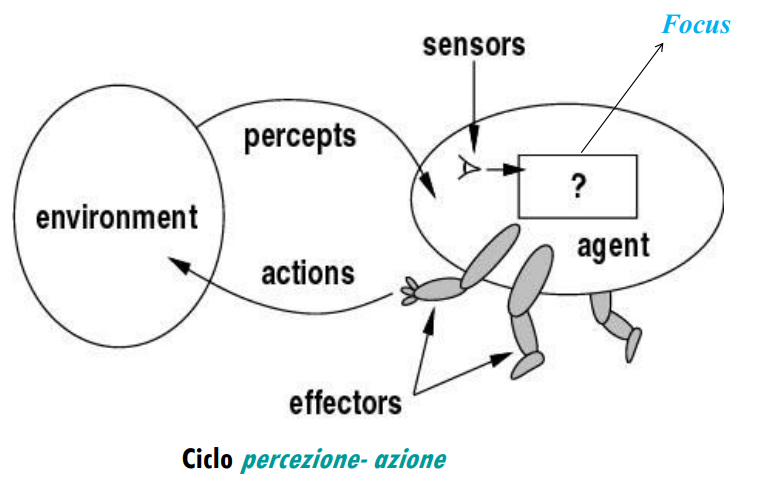
\includegraphics[width=0.7\textwidth]{immagini/Agenti_intelligenti2.png}
	\caption*{Agente intelligente}
\end{figure}
\subsection{Percezioni e azioni}
\begin{itemize}
	\item Percezione:\ input da sensori
	\item \textbf{Sequenza percettiva}:\ \textit{storia completa delle percezioni}
\end{itemize}
La scelta dell'azione è funzione unicamente della sequenza percettiva.

\textbf{Funzione agente}:\ definisce l'azione da compiere per ogni seguenza percettiva (descrive completamente l'agente).
\begin{center}
	\textit{Sequenza percettiva} $\rightarrow$ \textit{Azione}
\end{center}
Implementata da un \textbf{programma agente}.\
Il compito (IA) è progettare il \textit{programma agente}.
\begin{figure}[H]
	\centering
	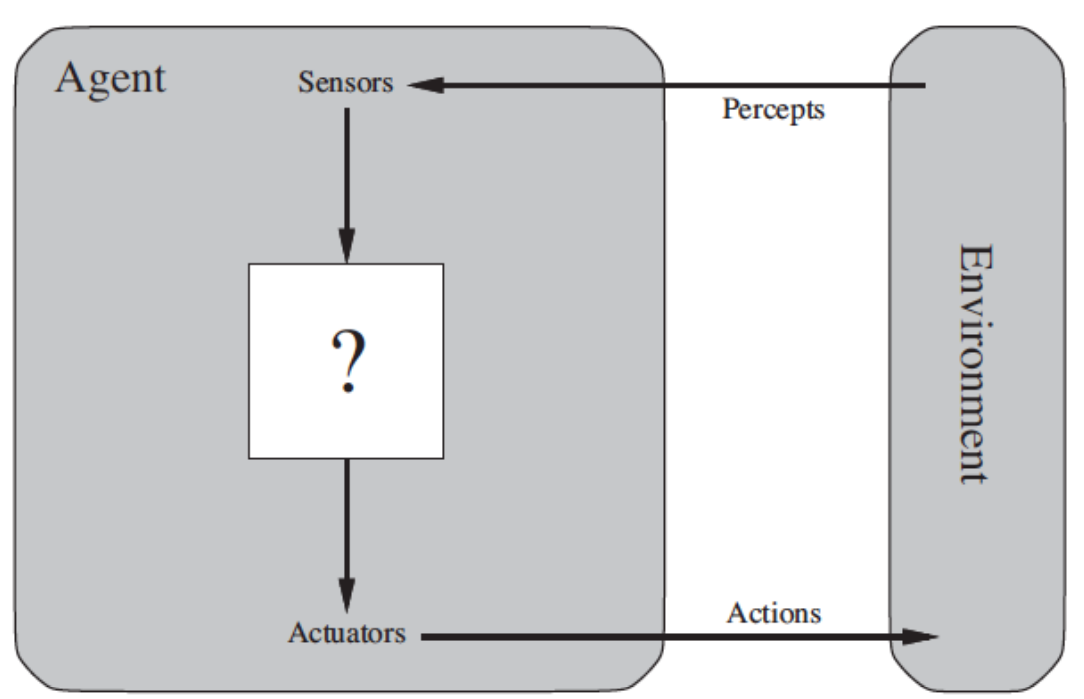
\includegraphics[width=0.6\textwidth]{immagini/Agente.png}
	\caption*{Agente e ambiente:\ architettura astratta}
\end{figure}
\subsection{Agenti razionali}
Un \textbf{agente razionale} interagisce con il suo ambiente in maniera ``efficace'' (fa la cosa ``giusta'').\

Serve un criterio di \textbf{valutazione} oggettivo dell'effetto delle azioni dell'agente (della sequenza di stati dell'ambiente).

\subsubsection{Valutazione della prestazione}
Misura di prestazione
\begin{itemize}
	\item Esterna (come vogliamo che il mondo evolva?)
	\item Scelta dal progettista a seconda del problema considerando l'effetto desiderato sull'ambiente
	\item (possibile) Valutazione su ambienti diversi
\end{itemize}

\subsubsection{Agente razionale:\ definizione}
La razionalità è relativa a (dipende da):
\begin{itemize}
	\item la misura di prestazioni,
	\item le conoscenze pregressa dell'ambiente,
	\item le percezioni presenti e passate (seq.\ percettiva),
	\item le capacità dell'agente (azioni possibili).
\end{itemize}

\vspace{12pt}
\noindent\textbf{Agente razionale}:\ per ogni sequenza di percezioni compie l'azione che \textit{massimizza il valore atteso della misura delle prestazioni}, considerando le sue percezioni passate e la sua conoscenza pregressa.

\noindent\textbf{Razionalità non onniscienza}:\ non si pretendono perfezione e conoscenza del ``futuro'', ma massimizzare il risultato atteso.\ La scelta dell'azione è \textit{funzione unicamente} della sequenza percettiva:\ potrebbero essere necessarie azioni di acquisizione di informazioni o esplorative.

\noindent\textbf{Razionalità non onnipotenza}:\ le capacità dell'agente possono essere limitate.

\subsubsection{Razionalità e apprendimento}

Raramente tutta la conoscenza sull'ambiente può essere fornita ``a priori'' dal programmatore, quindi l'agente razionale deve essere in grado di modificare il proprio comportamento con l'esperienza (le percezioni passate):\ può migliorare esplorando, \textit{apprendendo}, aumentando autonomia per operare in ambienti differenti o mutevoli.

\subsubsection{Agenti autonomi}

\textbf{Agente autonomo}:\ un agente è autonomo nella misura in cui il suo comportamento dipende dalla sua esperienza.\
Un agente il cui comportamento fosse determinato solo dalla sua conoscenza \textit{built-in}, sarebbe non autonomo e poco flessibile (\textit{comportamento stereotipato}).

\subsection{Ambienti}
Definire un problema per un agente significa caratterizzare l'ambiente in cui l'agente opera (ambiente operativo).\
Agente razionale $\rightarrow$ soluzione.\

Descrizione \textbf{PEAS} dei problemi
\begin{itemize}
	\item \textbf{P}erformance:\ prestazione
	\item \textbf{E}nvironment:\ ambiente
	\item \textbf{A}ctuators:\ attuatori
	\item \textbf{S}ensors:\ sensori
\end{itemize}

\begin{figure}[H]
	\centering
	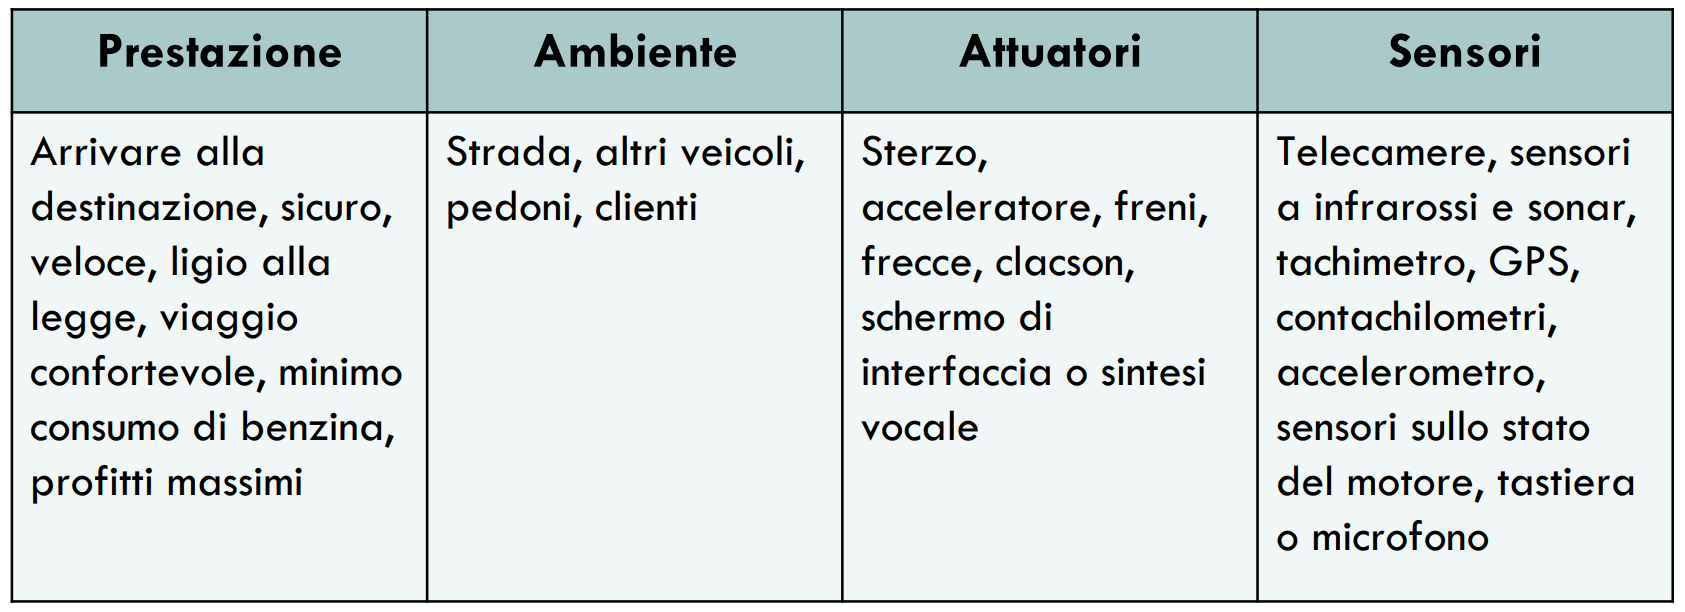
\includegraphics[width=0.9\textwidth]{immagini/Ambiente_Taxi.png}
	\caption*{Esempio:\ agente guidatore di taxi.}
\end{figure}

\subsubsection{Proprietà dell'ambiente-problema}
\begin{itemize}
	\item Completamente/parzialmente osservabile
	\item Agente singolo/multi-agente
	\item Deterministico/stocastico/non deterministico
	\item Episodico/sequenziale (esiste storia?)
	\item Statico/dinamico
	\item Discreto/continuo
\end{itemize}

\subsubsection{Osservabilità}

Ambiente \textbf{completamente osservabile}:\ l'apparato percettivo è in grado di dare una conoscenza completa dell'ambiente o almeno tutto quello che serve a decidere l'azione.\
Non c'è bisogno di mantenere uno stato del mondo (esterno).\\
Ambiente \textbf{parzialmente osservabile}:\ sono presenti limiti o inaccuratezze dell'apparato sensoriale.

\subsubsection{Ambiente singolo/multiagente}
\textbf{Distinzione agente/non agente}:\ il mondo può anche cambiare per eventi, non necessariamente per azioni di agenti.\\
Ambiente \textbf{multi-agente competitivo} (schacchi):\ comportamento randomizzato (è razionale).\\
Ambiente \textbf{multi-agente cooperativo} (o benigno):
\begin{itemize}
	\item Stesso obiettivo
	\item Comunicazione
\end{itemize}

\subsubsection{Predicibilità}
\textbf{Deterministico}:\ se lo stato successivo è completamente determinato dallo stato corrente e dall'azione.\
Esempio:\ scacchi.\\
\textbf{Stocastico}:\ esistono elementi di incertezza con associata probabilità.\
Esempi:\ guida, tiro in porta.\\
\textbf{Non deterministico}:\ si tiene traccia di più stati possibili risultato dell'azione (ma non in base ad una probabilità).

\subsubsection{Episodico/sequenziale}
\textbf{Episodico}:\ l'esperienza dell'agente è divisa in episodi atomici indipendenti.\
In ambienti episodici non c'è bisogno di pianificare.\\
\textbf{Sequenziale}:\ ogni decisione influenza le successive.

\subsubsection{Statico/dinamico}

\textbf{Statico}:\ il mondo non cambia mentre l'agente decide l'azione.\\
\textbf{Dinamico}:\ cambia nel tempo, va osservata la contingenza.\
Tardare equivale a non agire.\\
\textbf{Semi-dinamico}:\ l'ambiente non cambia ma la valutazione dell'agente sì.\
Esempio:\ scacchi con timer.

\subsubsection{Discreto/continuo}

Possono assumere valori discreti o continui
\begin{itemize}
	\item lo stato:\ solo un numero finito di stati;
	\item il tempo;
	\item le percezioni;
	\item le azioni.
\end{itemize}
La guida del taxi è un problema con stato e tempo continui\dots

Combinatoriale (nel discreto) versus infinito (nel continuo).

\subsubsection{Noto/ignoto}
Distinzione riferita allo stato di conoscenza dell'agente sulle leggi fisiche dell'ambiente.\
L'agente conosce l'ambiente oppure deve compiere azioni esplorative?

Noto è diverso da osservabile (e.g.\ carte coperte, regole note).

\textit{Ambienti reali}:\ parzialmente osservabili, stocastici, sequenziali, dinamici, continui, multi-agente, ignoti.

\subsubsection{Simulatore di ambienti}

Uno strumento software che si occupa di:
\begin{itemize}
	\item generare stimoli per gli agenti,
	\item raccogliere le azioni in risposta,
	\item aggiornare lo stato dell'ambiente,
	\item attivare altri processi che influenzano l'ambiente,
	\item valutare le prestazioni degli agenti.
\end{itemize}
Esperimenti su classi di ambienti (variando le condizioni) essenziale per valutare capacità di generalizzare.\
Valutazione prestazione come medie su più istanze.

\subsection{Struttura di un agente}
Agente = Architettura + Programma

\begin{center}
	Agente: Percezioni $\rightarrow$ Azioni
\end{center}
Il \textbf{programma dell'agente} implementa la funzione \textit{Agente}.

\subsubsection{Programma agente}
\textbf{function} Skeleton-Agent (\textit{percept}) \textbf{returns} \textit{action}

\textbf{static}:\ \textit{memory}, the agent's memory of the world

\textit{memory} $\leftarrow$ UpdateMemory(\textit{memory}, \textbf{percept})

\textit{action} $\leftarrow$ Choose-Best-Action(\textit{memory})

\textit{memory} $\leftarrow$ UpdateMemory(\textit{memory}, \textbf{action})

\textbf{return} \textit{action}

\subsubsection{Agente basato su tabella}

La scelta dell'azione è un accesso a una tabella che associa un'azione ad ogni possibile sequenza di percezioni.\
Problemi:
\begin{enumerate}
	\item Dimensione:\ per giocare a scacchi servirebbe una tabella con un numero di righe $>>$ 10\textsuperscript{80} numero di atomi nell'universo! $\rightarrow$ ingestibile
	\item Difficile da costruire
	\item Nessuna autonomia
	\item Di difficile aggiornamento, apprendimento complesso.
\end{enumerate}

\noindent In IA vogliamo realizzare agenti razionali con programma ``\textit{compatto}''.

\subsubsection{Agenti reattivi semplici}
\textbf{function} Agente-Reattivo-Semplice (\textit{percezione}) \textbf{returns} \textit{azione}

\textbf{persistent}:\ \textit{regole}, un insieme di regole

condizione-azione (if-then)

\textit{stato} $\leftarrow$ Interpreta-Input(\textit{percezione})

\textit{regola} $\leftarrow$ Regola-Corrispondente(\textit{stato}, \textit{regole})

\textit{azione} $\leftarrow$ \textit{regola}.Azione

\textbf{return} \textit{azione}

\begin{figure}[H]
	\centering
	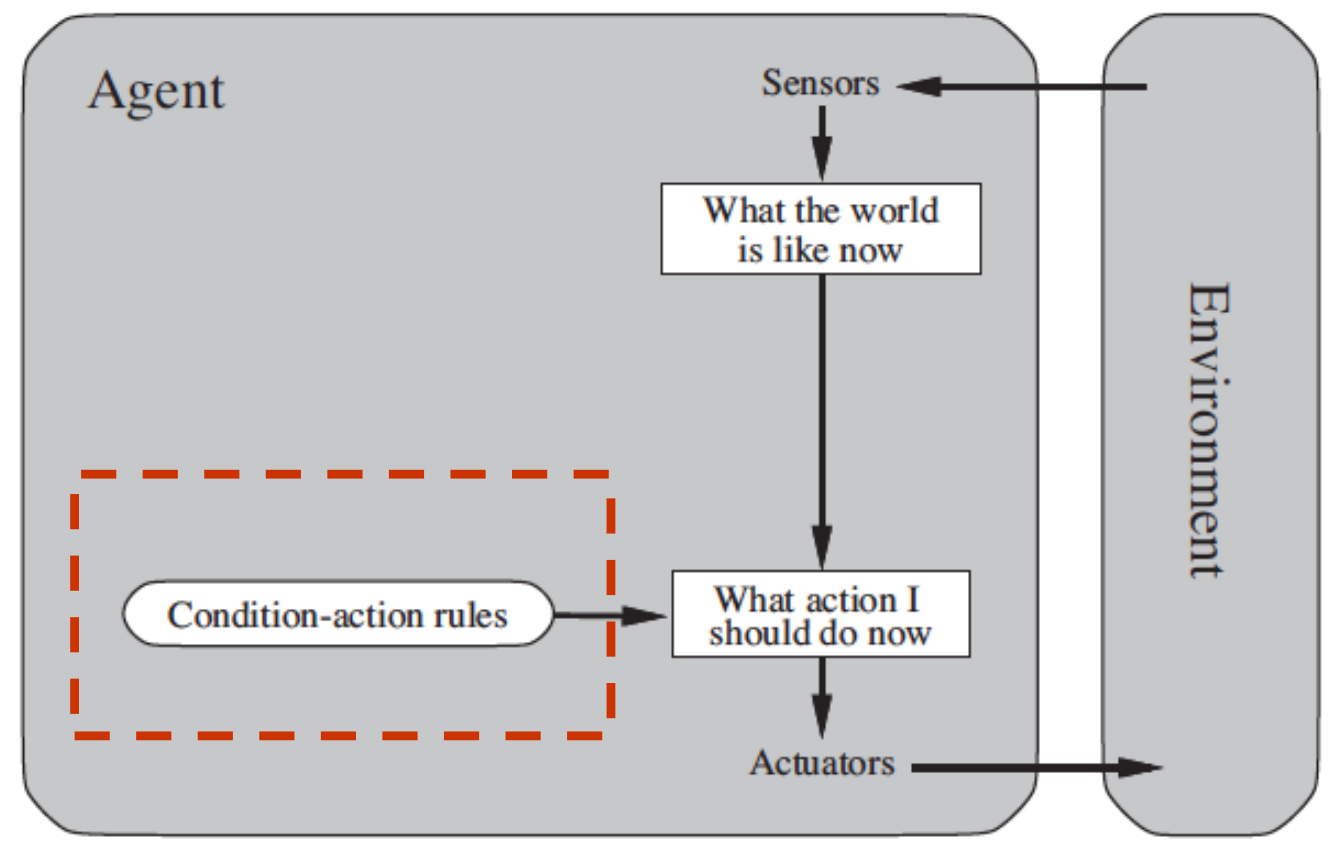
\includegraphics[width=0.5\textwidth]{immagini/Agenti_reattivi.png}
\end{figure}

\subsubsection{Agenti basati su modello}

\textbf{function} Agente-Basato-su-Modello (\textit{percezione}) \textbf{returns} \textit{azione}

\textbf{persistent}:\ \textit{stato}, una descrizione dello stato corrente

\qquad \qquad \qquad \textit{modello}, conoscenza del mondo

\qquad \qquad \qquad \textit{regole}, un insieme di regole condizione-azione

\qquad \qquad \qquad \textit{azione}, l'azione più recente

\textit{stato} $\leftarrow$ Aggiorna-Stato(\textit{stato}, \textit{azione}, \textit{percez}., \textit{modello})

\textit{regola} $\leftarrow$ Regola-Corrispondente(\textit{stato}, \textit{regole})

\textit{azione} $\leftarrow$ \textit{regola}.Azione

\textbf{return} \textit{azione}

\begin{figure}[H]
	\centering
	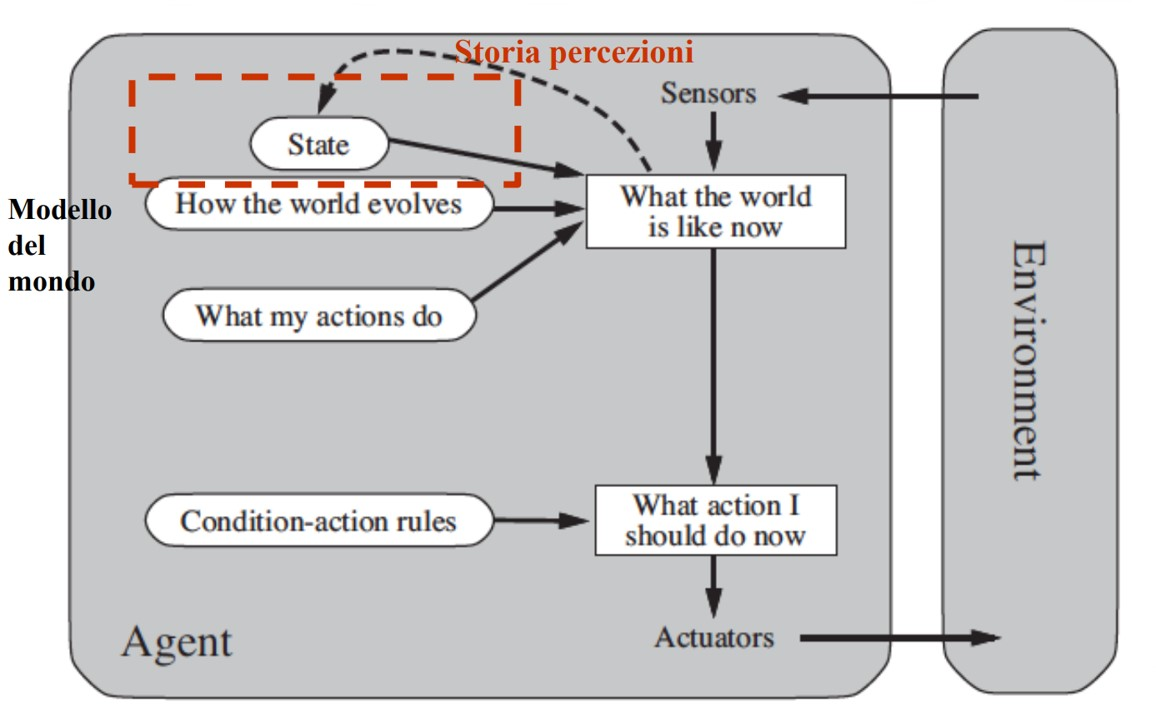
\includegraphics[width=0.5\textwidth]{immagini/Agenti_modelBased.jpg}
\end{figure}

\subsubsection{Agenti con obiettivo}

Sono guidati da un obiettivo nella scelta dell'azione (è fornito un goal esplicito, per esempio città da raggiungere).\

\begin{itemize}
	\item A volte l'azione migliore dipende da qual è l'obiettivo da raggiungere (es. da che parte devo girare?).
	\item Devono pianificare una sequenza di azioni per raggiungere l'obiettivo.
	\item Meno efficienti ma più flessibili di un agente reattivo (obiettivo può cambiare, non è già codificato nelle regole).
\end{itemize}

\begin{figure}[H]
	\centering
	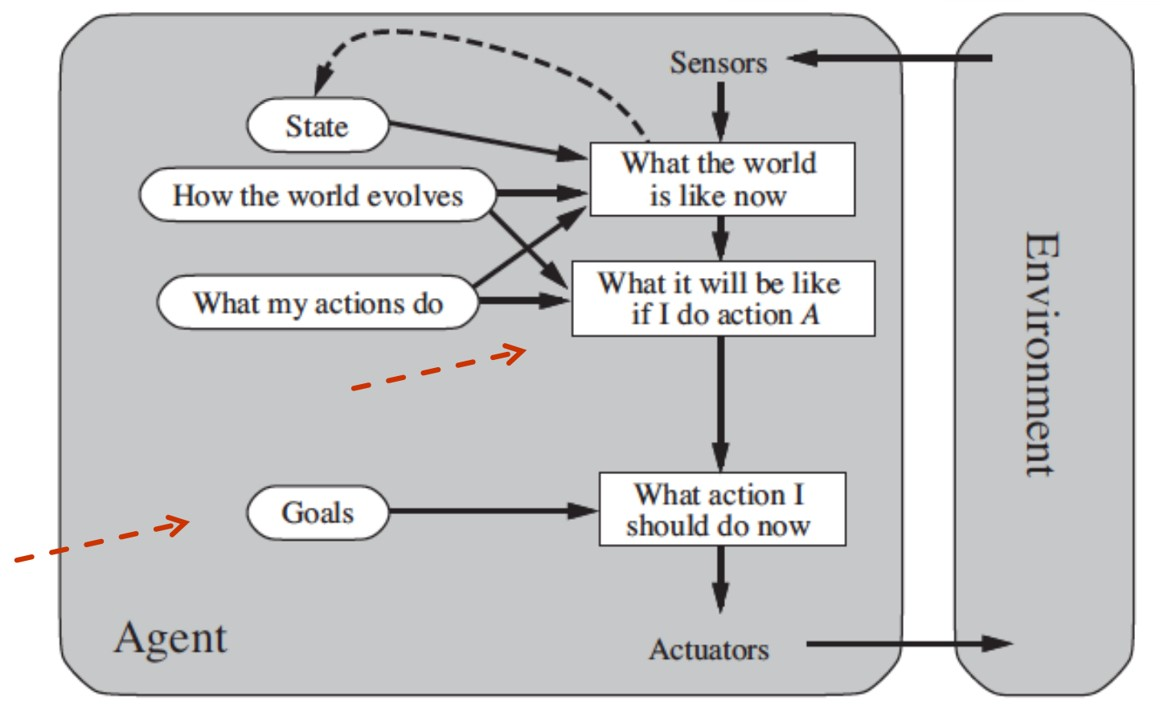
\includegraphics[width=0.6\textwidth]{immagini/Agente_obiettivo.jpg}
\end{figure}

\subsubsection{Agenti con valutazione di utilità}

Obiettivi alternativi (o più modi per raggiungerlo), l'agente deve decidere verso quali di questi muoversi.\
Necessaria una funzione di \textbf{utilità} (che associa ad uno stato obiettivo un numero reale).

Obiettivi più facilmente raggiungibili di altri, la funzione di utilità tiene conto anche della probabilità di successo (e/o di ciascun risultato):\ \textbf{utilità attesa} (o in media)

\begin{figure}[H]
	\centering
	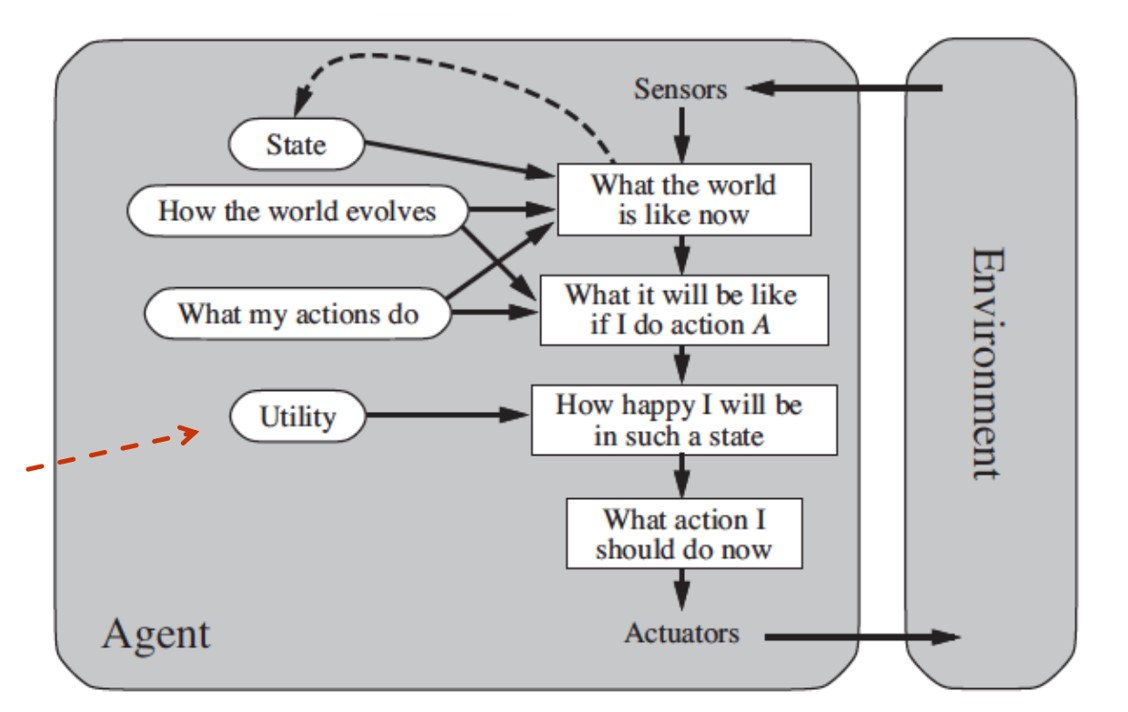
\includegraphics[width=0.5\textwidth]{immagini/Agente_utility.jpg}
\end{figure}

\subsubsection{Agenti che apprendono}
\begin{enumerate}
	\item Componente di apprendimento:\ produce cambiamenti al programma agente e ne migliora prestazioni, adattando i suoi componenti, apprendendo dall'ambiente.
	\item Elemento esecutivo:\ il programma agente
	\item Elemento critico:\ osserva e dà feedback sul comportamento
	\item Generatore di problemi:\ suggerisce nuove situazioni da esplorare
\end{enumerate}

\begin{figure}[H]
	\centering
	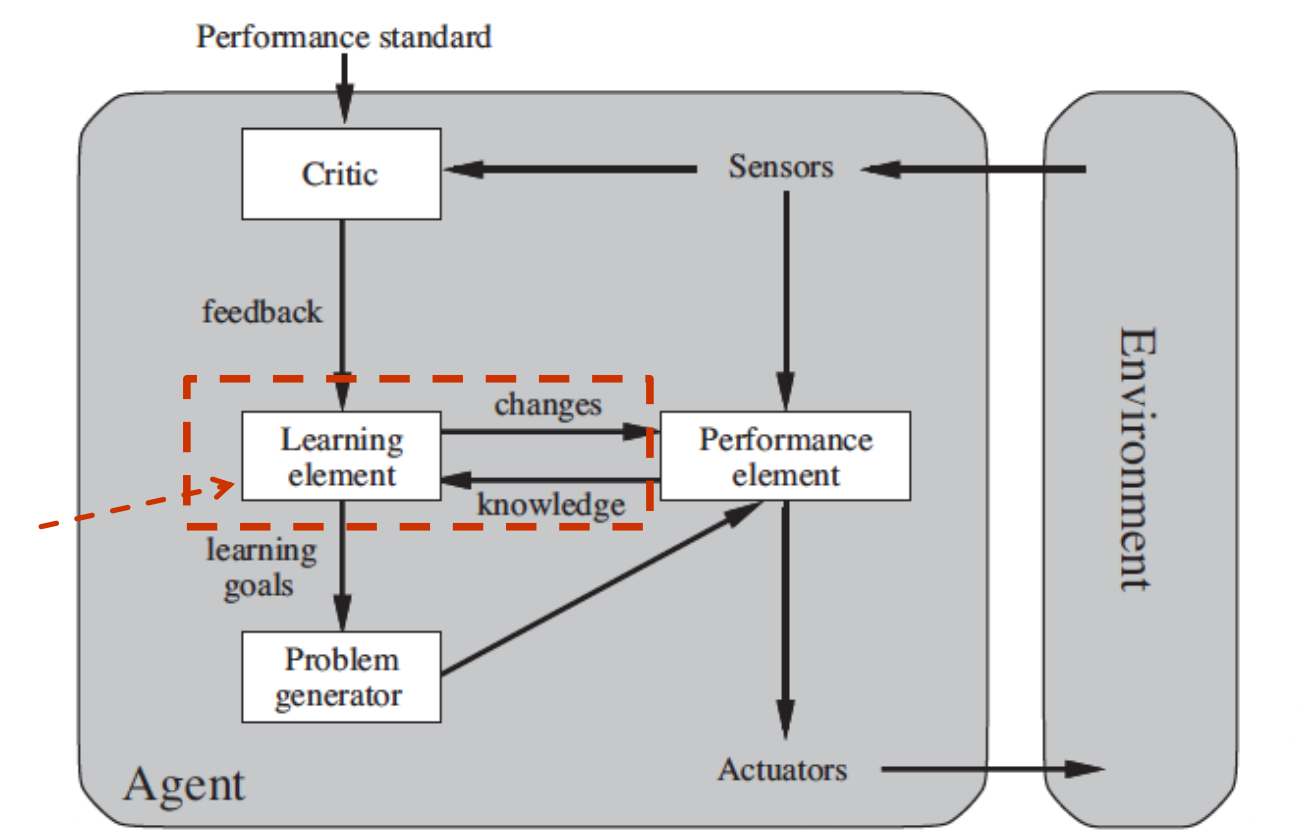
\includegraphics[width=0.5\textwidth]{immagini/Agente_apprende.png}
\end{figure}

\subsubsection{Tipi di rappresentazione}

\begin{itemize}
	\item Rappresentazione atomica (stati)
	\item Rappresentazione fattorizzata (piu variabili e attributi)
	\item Rappresentazione strutturata (aggiunge relazioni)
\end{itemize}

\begin{figure}[H]
	\centering
	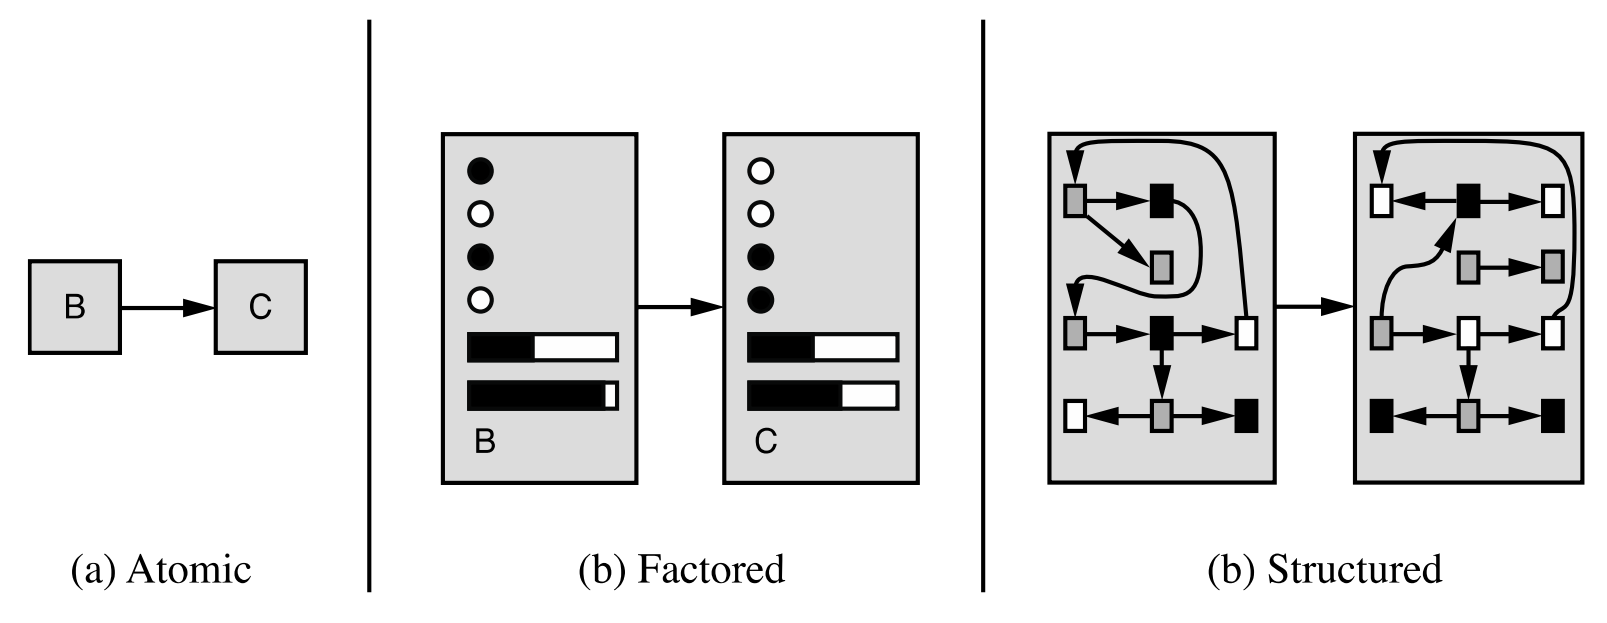
\includegraphics[width=\textwidth]{immagini/Tipi_rappresentazione.png}
\end{figure}
